\documentclass{article} % document class we use it to specify our document type
% if you want to change the font use this rule after documentclass tag ['size'pt]
\usepackage[utf8]{inputenc}
\usepackage[margin=1in]{geometry} % use this package for formatting. in here we change the size of margin to 1 inch.
\usepackage{hyperref} % this package allows us to make url links clickable.

%\usepackage[parfill]{parskip} % this package with this rule will begin a new paragraph by an empty line rather than an indent. it's commented cause i whant to use the default.

\usepackage{graphicx} % graphics package

% use this to create a continuing list
\usepackage{enumitem}

% for math symbols
\usepackage{amssymb}

% algorithm environment package
\usepackage{algpseudocode}

% this is how you can add two or more packages at once
\usepackage{caption,subcaption}

 % for our multirow table
\usepackage{multirow}

% this package allows us to tab few spaces in the document.
\usepackage{tabto}

% these three will always be there
\title{\LaTeX \space basics}
\author{pouya ardehkhani}
\date{} % you can specify the date or leave it empty for no date. it is removable cause the compiler will put it there

% what we write is always between the begin and end tag
% we always have one of them with the type {document}
% remember a begin tag always end with a end tag with that type
\begin{document}
% we always do this to create out title and author
\maketitle

% creating a table of content
\tableofcontents
% for going to next page
\pagebreak
% use this tag to create an section
\section{Introduction}
    \LaTeX is a software system for document preparation. When writing, the writer uses plain text as opposed to the formatted text found in "What You See Is What You Get" word processors like Microsoft Word, LibreOffice Writer and Apple Pages. The writer uses markup tagging conventions to define the general structure of a document (such as article, book, and letter), to stylise text throughout a document (such as bold and italics), and to add citations and cross-references. A TeX distribution such as TeX Live or MiKTeX is used to produce an output file (such as PDF or DVI) suitable for printing or digital distribution.
    
    It's widely used in academia for the communication and publication of scientific documents in many fields, including mathematics, computer science, engineering, physics, chemistry, economics, linguistics, quantitative psychology, philosophy, and political science. It also has a prominent role in the preparation and publication of books and articles that contain complex multilingual materials, such as Sanskrit and Greek. \LaTeX uses the TeX typesetting program for formatting its output, and is itself written in the TeX macro language.

    % next paragraph by default indented we can change that by the help of packages
    
\section{Start}
    It's good to use a template if your not completely understand LaTeX but if you do you can upgrade it. You can see the source file to understand what we are talking about during this document. The important tags are commented so you can understand which tag must be in \LaTeX \space source file. \textbf{ALways remember to see the source file cause there is some symboles that we covered by commenting so we wont talk about them here.} use \textbf{two back slashes} to specify a new line explicitly.
    
    
    One of the best places to start is overleaf online LaTeX editor.  
     
    % use noindent tag to not to indent the new paragraph
    \noindent Access by this link \url{https://www.overleaf.com/}
    
    % \LaTeX tag will write LaTeX on its proper ways
    % use \space to insert an extra space
    \subsection{Sections}
        Use section tag to create a section. Also note that indenting in the source file don't matter and use percentage symbole to comment in the source file. Also remember that a tag in \LaTeX \space always start by a Back Slash.
        \subsubsection{Sub Sections}
            Also sub sections come with the subsection tag and for further sub sections just add another sub in subsection tag. 

\section{Packages}
    I know that it's to soon to talk about it but because we already used it so I thought it's better to dive a little into it but remember we can't cover all the packages so you can google it or ... to find out about different packages. Packages are like programming language library that gives us some useful tools.
    
    \noindent We use the usepackage tag to use a package. There are different packages and also packages can come with an input command [ ] right after the usepackage tag.
    
    \noindent One of the packages we use wildly called geometry that allows us formatting the document. We used it to change the margin of our document.

    \subsection{Useful Methods}
        use geometry{landscape} tag will set the doc to be in landscape mode.
        
        \noindent use graphicx package to handle graphical data.
    
        \noindent use the amssymb package for math symbols.
        
        \noindent use the epstopdf package to convert eps graphics to pdf graphics.
    
        \noindent you can search fo more packages online.
    
\section{Basic Formatting}

    % we will talk about this table number manipulating. 
    \begin{enumerate}
        \item Emphasis on something  
        
        % use the tag bellow to have a tab space size.  but it has large problem so dont use tab tag. use the \quad or \qquad tag instead.
        \qquad We can bold a tex with textbf tag \textbf{ like this } remember bolding will only happen in curly braces.
    \end{enumerate}
        
 
    
    \begin{enumerate}[resume]
        \item Italic Tag
        
        \qquad We can italic a part of text \emph{like this}
    \end{enumerate}
    

    
    \begin{enumerate}[resume]
        \item Underline
        
        \qquad We can underline a \underline{text like this}
    \end{enumerate}
    
    
    \noindent NOTE:
    
    formatting only applies to the text in curly braces.
    
    \begin{enumerate}[resume]
        \item Paragraph Formatting 
        
        \qquad If you saw the source file you will notice the noindent tag which makes the new paragraphs not to be indented.
    \end{enumerate}
    
        
    \begin{enumerate}[resume]
        \item Oddities
        
        \qquad quoting there are two options first like normal keyboard key 'like' , "this" but something is odd for properly declare them use the  quoting key in left of your keyboard `like' , ``this".
        
    \end{enumerate}
    
    
    \begin{enumerate}[resume]
        \item Font
        
        \qquad see this link for more informations \url{https://www.overleaf.com/learn/latex/Font_typefaces}.
        
    \end{enumerate}
    
    
\section{List Structures}

NOTE:

Pay attention to the source file. Also list are like an environment so the must begin and end with begin and end tag.

    % this is a nested environment
    %\begin{enumerate} this command and the edn tag(\end{enumerate}) will be specify by { } that which type of environment we need.
    \begin{enumerate}
        \item Numbered List

        \qquad We already see one type of list called enumerated list in section 4. We used item tag to add items to our list.
        
        \item Bulleted List
        
            \begin{itemize}
                \item like this.
                
                \qquad you can write anything here.
            \end{itemize}
            
       \item Description List
       
            \begin{description}
                
                % at [ ] write the text that you want to give a description about it. it will be bolded automatically.
                \item[\LaTeX] software system for document preparation.
            
            \end{description}
            
        \item Nested Environment
        
            \qquad in this section we already showed you how to create a nested environment.
        
    \end{enumerate}
 
 
 
    
% If you simply want the character to be printed just as any other letter, include a \ in front of the character.
\section{Table \& Floats}   

\begin{itemize}
    \item Tabular Environment
    
        Use begin and end tag with {tabular} to create a tabular environment. use another {} to specify number of columns and their align type and vertical bar. use | (SHIFT + BACKSLASH ) to specify a vertical bar. use l for left align type and c for centered . like this:
    
    % for making it to not be like sticking to the last sentence use this options
    
    %\vspace{.5cm} % this tag add 0.5 cm skip between paragraphs
    \smallskip % this tag skips a little
    %\bigskip % this tag skips a large amount.
    \begin{tabular}{| l | c |}
        % we use \hline for horizontal bar.
        % use the & to go at the next column.
        % for finishing with a row use \\ at the end.
        \hline
        first & second\\
        \hline
        third & four\\
        \hline
        
    \end{tabular}
    
    \smallskip
    \noindent for double bars use hline tag twice and add double backslashes between columns. 
    
    
    
    %\vspace{.5cm} % this tag add 0.5 cm skip between paragraphs
    \smallskip % this tag skips a little
    %\bigskip % this tag skips a large amount.
    \begin{tabular}{| l || c |}
        % we use \hline for horizontal bar.
        % use the & to go at the next column.
        % for finishing with a row use \\ at the end.
        \hline \hline
        first & second\\
        \hline \hline
        third & four\\
        \hline \hline
        
    \end{tabular}
    
\end{itemize}



\begin{itemize}
    \item Table
    
    \smallskip
    Table it's a floating environment (float = \LaTeX \space choose where to put it)
    
    % [ ] in there we specified where to put it only Approximately.
    % h for here
    % t for top
    % b for bottom
    % p for separate page
    % if they come sequentially, they are places that our table can be there
    \begin{table}[htb]
        % instead of \begin{center} we use this tag to make every thing centers
        \centering
        \begin{tabular}{c|c}
         first    &    second\\
        \hline
         third    &    fourth
        \end{tabular}
        
        % use this tag for caption in a table
        \caption{this is a table}
        % use label tag for referencing a table 
        \label{tab:table}
    \end{table}
    
    % use ~ to use the number and table together
    % use the \ref tag to make a reference
    this is a references to table~\ref{tab:table}
    
    % we can add also another environment in it.
    
\end{itemize}

\section{Graphics}

    for including a picture use this tag.
    
    % use [ ] for specifying size (width , length)
    % remember {name.format}
    
\includegraphics[width=2in]{latex.png}

    \subsection{Graphic Float Figure}
    
        we can use it to reference it.
        
        \begin{figure}[htbp]
            \centering
            
\includegraphics[width=2in]{latex.png}
            % new caption
            \caption{Caption}
            % label
            \label{fig:my_label}
        \end{figure}
        
    \noindent we will talk about more about graphics later.
    
    
    
\section{BibTeX References and Citations}

    we use the bib file for citations.
    
    I read an article~\cite{ali2012}. I read a book~\cite{kim2006}. I visited this site~\cite{site}.
    
    % we use bibliography tag and bibliographystyle tag to include our bib file.
    % sorting depends on the style of our bib file. plain style will sort by author.
    \bibliographystyle{plain}
    \bibliography{bibtex}
    
    in other softwares might see a [?] on pdf you should see the console for warning. mostly you must re run again(you can fixit by using a online editor like overleaf). if you see bbl file it's output file of our bib file. 
    
    you can also referencing by mendelay application. you can search it for more info.
    
    \noindent NOTE:
    
        you can put thousand items in the bib file but only some of it will be put in the document that are already referenced.
    
    
\section{Mathematical Symbols and Equations}  

    to create a math environment use \$ math eq \$ to create a math environment.
    
    for more symbols you can search each. they most are tags but some of them are not tags.
    
    \smallskip
    
    % A \ is produced by typing $\backslash$
    \begin{tabular}{| c | c |}
        % we use \hline for horizontal bar.
        % use the & to go at the next column.
        % for finishing with a row use \\ at the end.
        \hline
        leg & less than or equal\\
        \hline
        geq & greater than or equal\\
        \hline
        \^{} & power\\
        \hline
        * & times\\
        \hline
        cup & union symbole\\
        \hline
        alpha & lowercase alpha\\
        \hline
        exists & the exist character\\
        \hline
        rightarrow & right arrow\\
        \hline
        gets & left arrow\\
        \hline
        
    \end{tabular}
    \smallskip
    
    % use \^{} to write a ^
    you can search the internet for more symbols
    
    \noindent examples
    
    here are some of the math equations. $a^{2} , b=5 , a*b=8$ , this is inline.
    
    % it's a floating environment. can be referenced by a label.
    \begin{equation}[htbp]
        2^3+6*12 \leq 11 \cup X \alpha 25 \exists 5 \rightarrow
    \label{eq:name}    
    \end{equation}
    
    
\section{Algorithms and Pseudocode}    
    
    
    there are multiple environment and packages but we choose algpseudocode package. note that this is just a preview or a brief, for more info search the internet. see the source file to understand how to write.
    
    % in \IF{math or text is allowed}. remember to end it when your done.
    \begin{algorithmic}
        \If{$A=B$}
            \State $A \gets 10$
            \State continue 
        \Else
            \While{$A!=5$}
                \State $A \gets A*B+(A-B)$
                \State A++
            \EndWhile
        \EndIf
    
    \label{alg:my_alg}
    \end{algorithmic}


\section{Sty Files}

    usually for journals and others. journals have their own style and class files which makes it easy to typeset your doc without even having to read the requirements!
    
    \noindent an example for style files can be found in this link: \\ \url{https://www.ieee.org/conferences/publishing/templates.html}
    
    within their zip file there is also some tex file that have lots of comments, which packages we can use and more. we can also just change the section for our writing so it's useful and we dont need to read the requirements we just change the text in it.
    
    
\section{Advance Feature for Tables and Graphics}
    
    \begin{itemize}
        \item FOR TABLES
        
        use the package multirow to create this tables:
        
        \begin{table}[htbp]
            \centering
            % use p{size} for size of a specified column.
            \begin{tabular}{| l | c | p{3cm} |}
            
            \hline
                cs135 & C++ & this is a specified size column\\
            \hline
                cs235 & java & \\
            \hline
            
            \end{tabular}
            \caption{specific column size}
            \label{tab:text wrapping}
        \end{table}
        
        multicolumn and multirow table :
        
        \begin{table}[htbp]
            \centering
            % use p{size} for size of a specified column.
            \begin{tabular}{| c | c | c |}
            
            \hline
                % \multicolumn{num of columns you want}{align (insert | for a bar)}{text}
                & \multicolumn{2}{c|}{RANGES} \\
            \hline
                & X & Y \\
            \hline
                % \multirow{num of rows}{width of columns(size)}{text}
                % * in here means natural or normal width of columns
                \multirow{2}{*}{xy} & 5 & 6 \\
                % first & cause it's already fill with \multirow tag
                & 2 & 4 \\
            \hline
            
            \end{tabular}
            \caption{muticolumn and multirow}
            \label{tab:muticolumn_and_multirow}
        \end{table}
        
        \item FOR GRAPHICS
        % use this tag change your graphic path
        % \graphicspath{{directory}}
        
        in source file I will show you how to create sub-figures:
        
        \qquad first we need to packages (caption-subcaption)
        
        \qquad note that you can also reference the sub-figures
        
        \qquad \% in here means end of one fegure and the next figure should be kept with this figure side by side
        
        \begin{figure}[h]
            \centering
            
                % \begin{subfigure}{place like tables}{size}
                % for size one of the commons is 0.num_of_subfig*\textwidth
                % \textwidth -> width of text in our doc 
                \begin{subfigure}[b]{0.2\textwidth}
                    \centering
                        % [] in here means scale you want
                        
\includegraphics[scale=0.3]{fig1.png}
                    \caption{sub fig 1}
                    \label{fig:sub1}
                \end{subfigure}%
                \begin{subfigure}[b]{0.2\textwidth}
                    \centering
                        % [] in here means scale you want
                        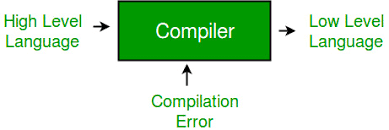
\includegraphics[scale=0.2]{fig2.png}
                    \caption{sub fig 2}
                    \label{fig:sub2}
                \end{subfigure}%

            \caption{sub figures}
            \label{fig:fig}
        \end{figure}

        now their references. this is figure~\ref{fig:fig}, this is the first sub-figure~\ref{fig:sub1}, this is the second sub-figure~\ref{fig:sub2}.
        
    \end{itemize}
    
\section{Separating Our Work in Multiple Files}
    
    use the input tag to have the text from a different file. no need for that file to have essential setups cause we have them right here but you can use package if you want to.
    
    % no need to type it's format
    \subsection{this is an imported subsection}

    this text belong to different file.
    
    
\section{Manipulating and Redefining Commands}

    there are few ways to cotrol the typesetting output.
    
    \noindent we already see how to make a continuing list in section 4 by help of a package.
    
    \noindent continuing list ---\textgreater \space every time we open an environment it starts counting order but we want to resume the counting from the last environment.


    \noindent another way do do it:
    
    \noindent by the help of the set counter tag we can do just like that.(no package needed) 

    \begin{enumerate}
        \item first
    \end{enumerate}
    
    % within the next list
    \begin{enumerate}
    
        % {enumi} means the first environment for nested environments use enumii or enumiii , ...
        % {1} means the number of the last count
        \setcounter{enumi}{1}
    
        \item second
    \end{enumerate}

    \noindent changing the numbering format for tables:
    
    \noindent use the renewcommand tag for changing some specific typeset settings.
    
    % before the list
    % {\theenumi} specific rule
    %{\Alph{enumi(nested environments are different)}} means number by capital(for lowercase use \alph{enumi} instead) alphabetic letters
    \renewcommand{\theenumi}{\Alph{enumi}}
    \renewcommand{\theenumii}{\Roman{enumii}}
    \begin{enumerate}
        \item one
        \item two
        \begin{enumerate}
            \item three
        \end{enumerate}
    \end{enumerate}
    
    \noindent for further knowledge visit this link \url{https://www.overleaf.com/learn/latex/Lists} 
    
    \noindent also for page numbering visit this link \url{https://www.overleaf.com/learn/latex/Page_numbering}

    % Inserts a blank space that will stretch accordingly to fill the space available.
    \hfill

    \noindent changing the bullets:
    
    % before the environment
    % {\labelitemi} this is it's rule
    % {$\rightarrow$} new bullet character
    \renewcommand{\labelitemi}{$\rightarrow$}
    \begin{itemize}
        \item see
    \end{itemize}
    
    there are lots of packages that allows us to change the typesetting output
    
\section{More Resources}   

    first you must know that most of the packages are found at CTAN site with docs.

    \renewcommand{\labelitemi}{$\bullet$}
    \begin{itemize}
        \item tabularx package
        
            \qquad let control over tabular environmrnt
        
        \item longtable package
        
            \qquad useful if you have a table that going to flow accross 2 pages. also you can determine whether or not that you have a header rowbon your table that is represented on the separate pages or does not repeat just appears once and then rest of the table flows onto another page.
        
        \item PSTricks
        
            \qquad let you to create graphics in latex
            
        \item templates
        
            \qquad you can visit this site for nice templates \url{https://www.latextemplates.com/}
            
        \item Additional Knowledge
        
            \qquad visit this site for learning new tricks
            
            \qquad \url{https://www.overleaf.com/learn}
        
    \end{itemize}
    
\end{document}
